\chapter{Amazon Web Services}

\section{Introdução}
A Amazon Web Services (AWS) é uma plataforma de serviços em nuvem segura, oferecendo poder computacional, armazenamento de banco de dados, distribuição de conteúdo e outras funcionalidades para ajudar as empresas em seu dimensionamento e crescimento. Segundo pesquisas recentes \cite{rightscale}, é o provedor de nuvem que detém a maior parcela do mercado em termos de adoção, com aproximadamente 64\%. Sua gama de serviços é bastante ampla, como mostrado abaixo:

\begin{figure}[h!]
  \centering
  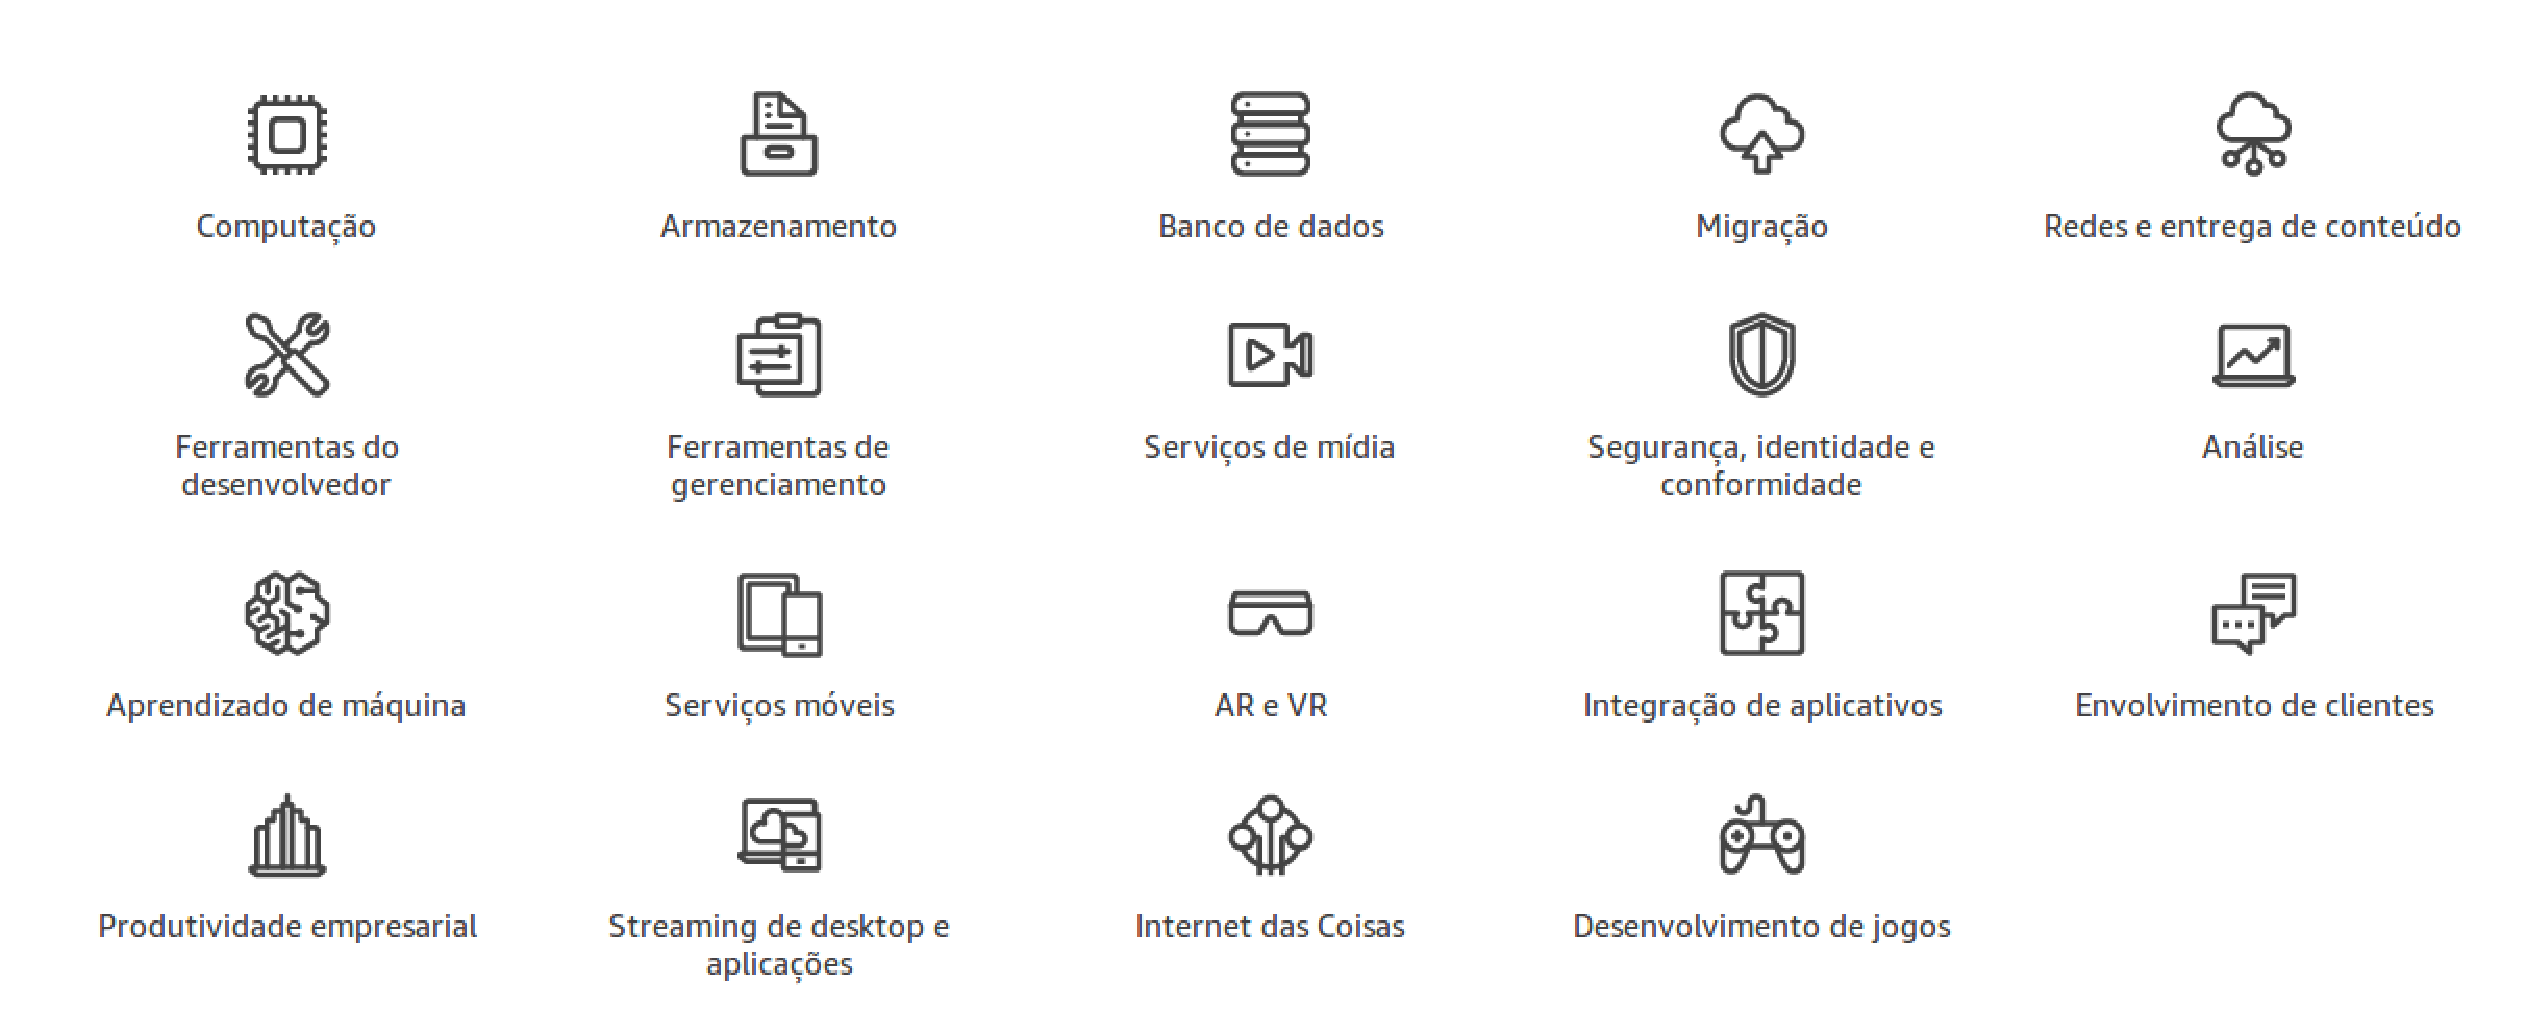
\includegraphics[scale=0.38]{imagens/aws-services.eps}
  \caption{Serviços da Amazon Web Services\cite{aws-services}}
\end{figure}

A AWS possui quatro serviços essenciais de nuvem para hospedagem de aplicações, sendo eles: \textbf{EC2}, \textbf{S3}, \textbf{RDS} e \textbf{Route 53}. Além disso, possui soluções para outros variados campos da computação, como inteligência artificial, desenvolvimento \textit{mobile}, realidade virtual e internet das coisas.


\section{Funcionamento básico}
No contexto do documento, serão destacados os quatro serviços já citados anteriormente:
jieaoshd

\begin{figure}[h!]
  \centering
  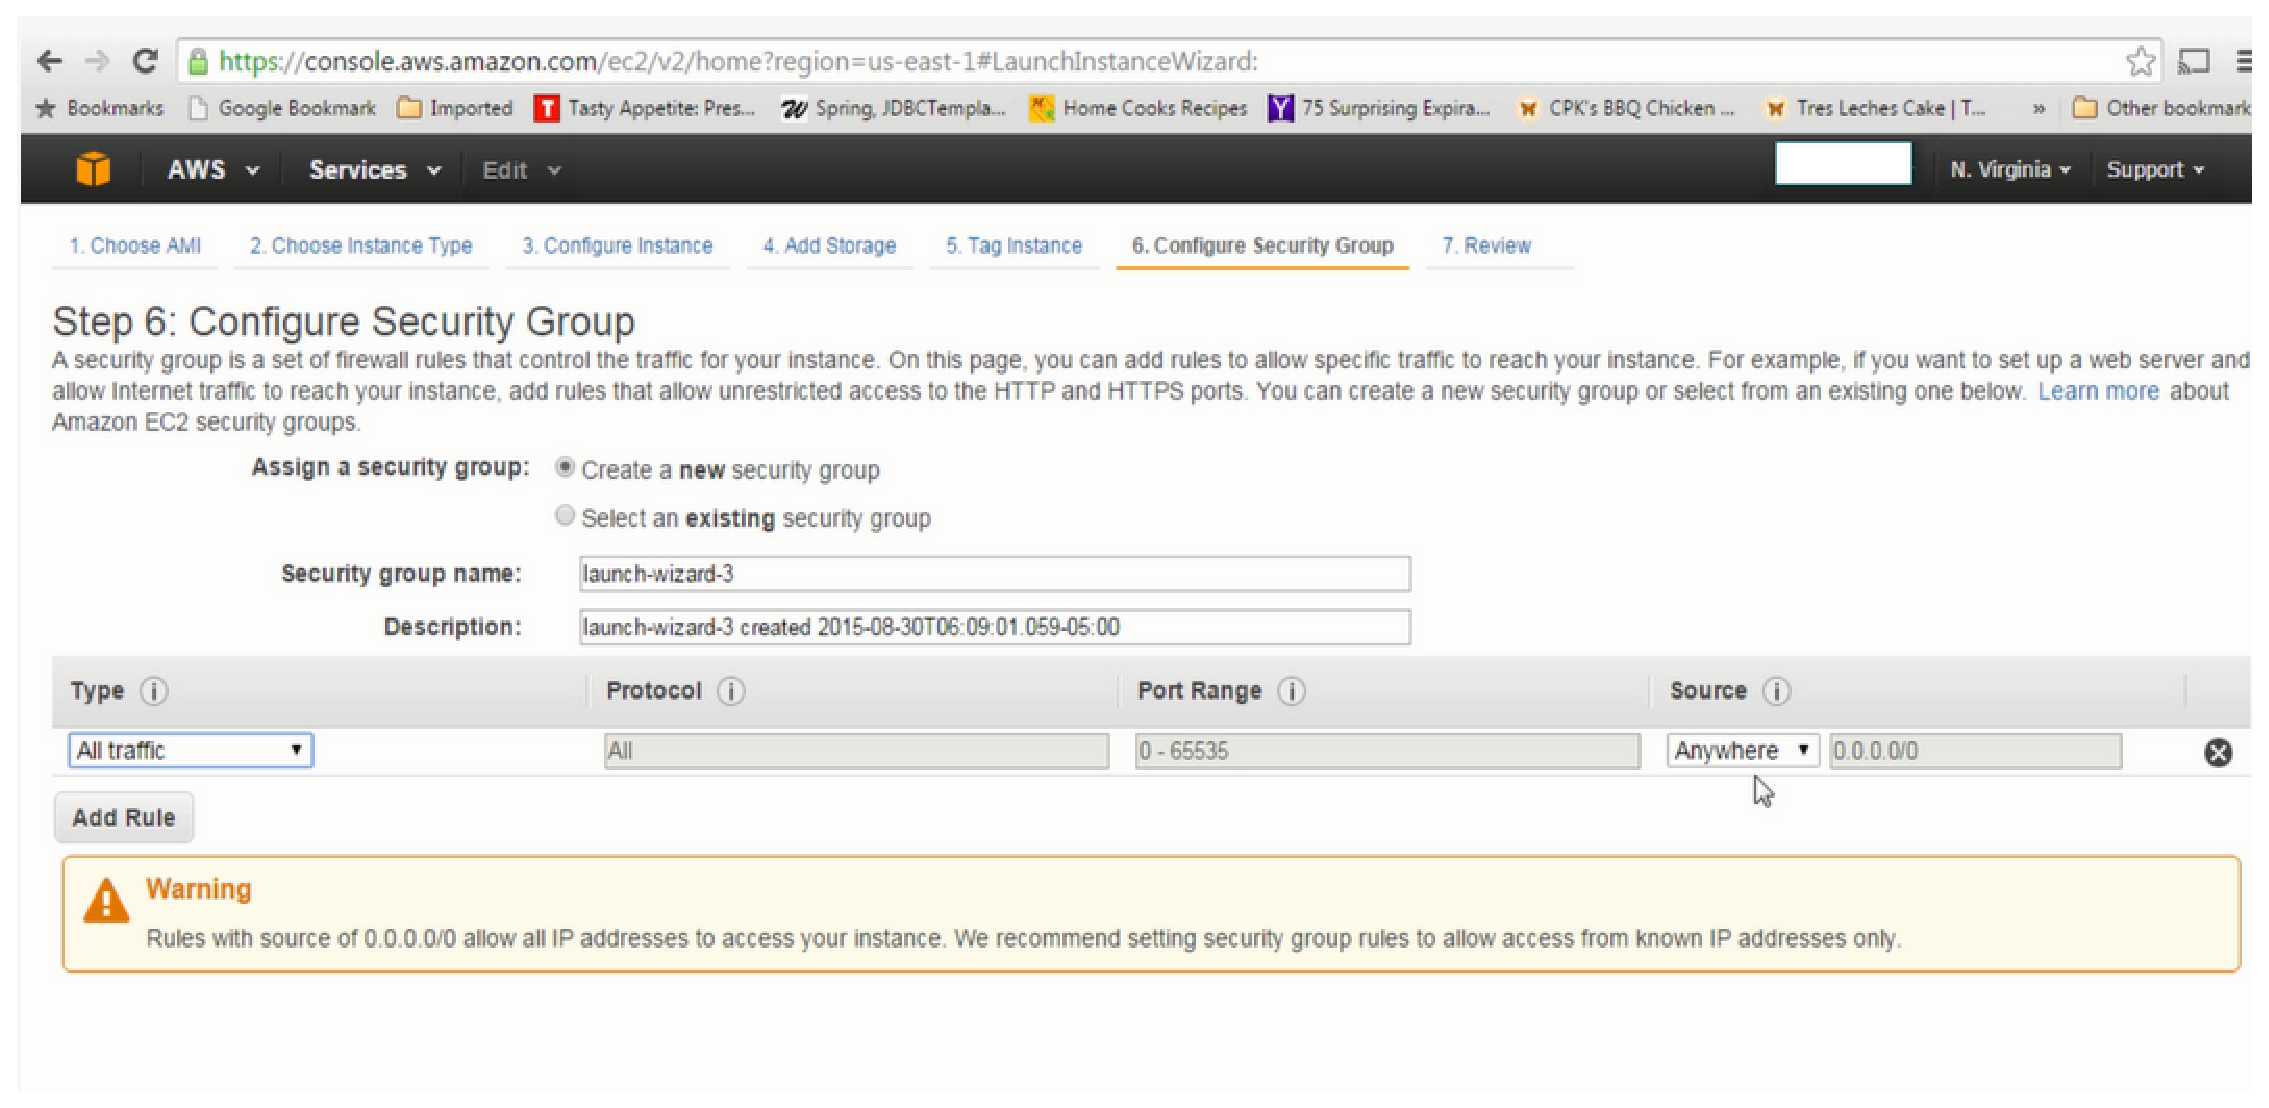
\includegraphics[scale=0.42]{imagens/aws-console.eps}
  \caption{Console da Amazon Web Services}
\end{figure}


\subsection{EC2}
\subsection{S3}
\subsection{RDS}
\subsection{Route 53}

\section{Outros Serviços}
\section{Conclusão}
